\begin{frame}
  \begin{center}
    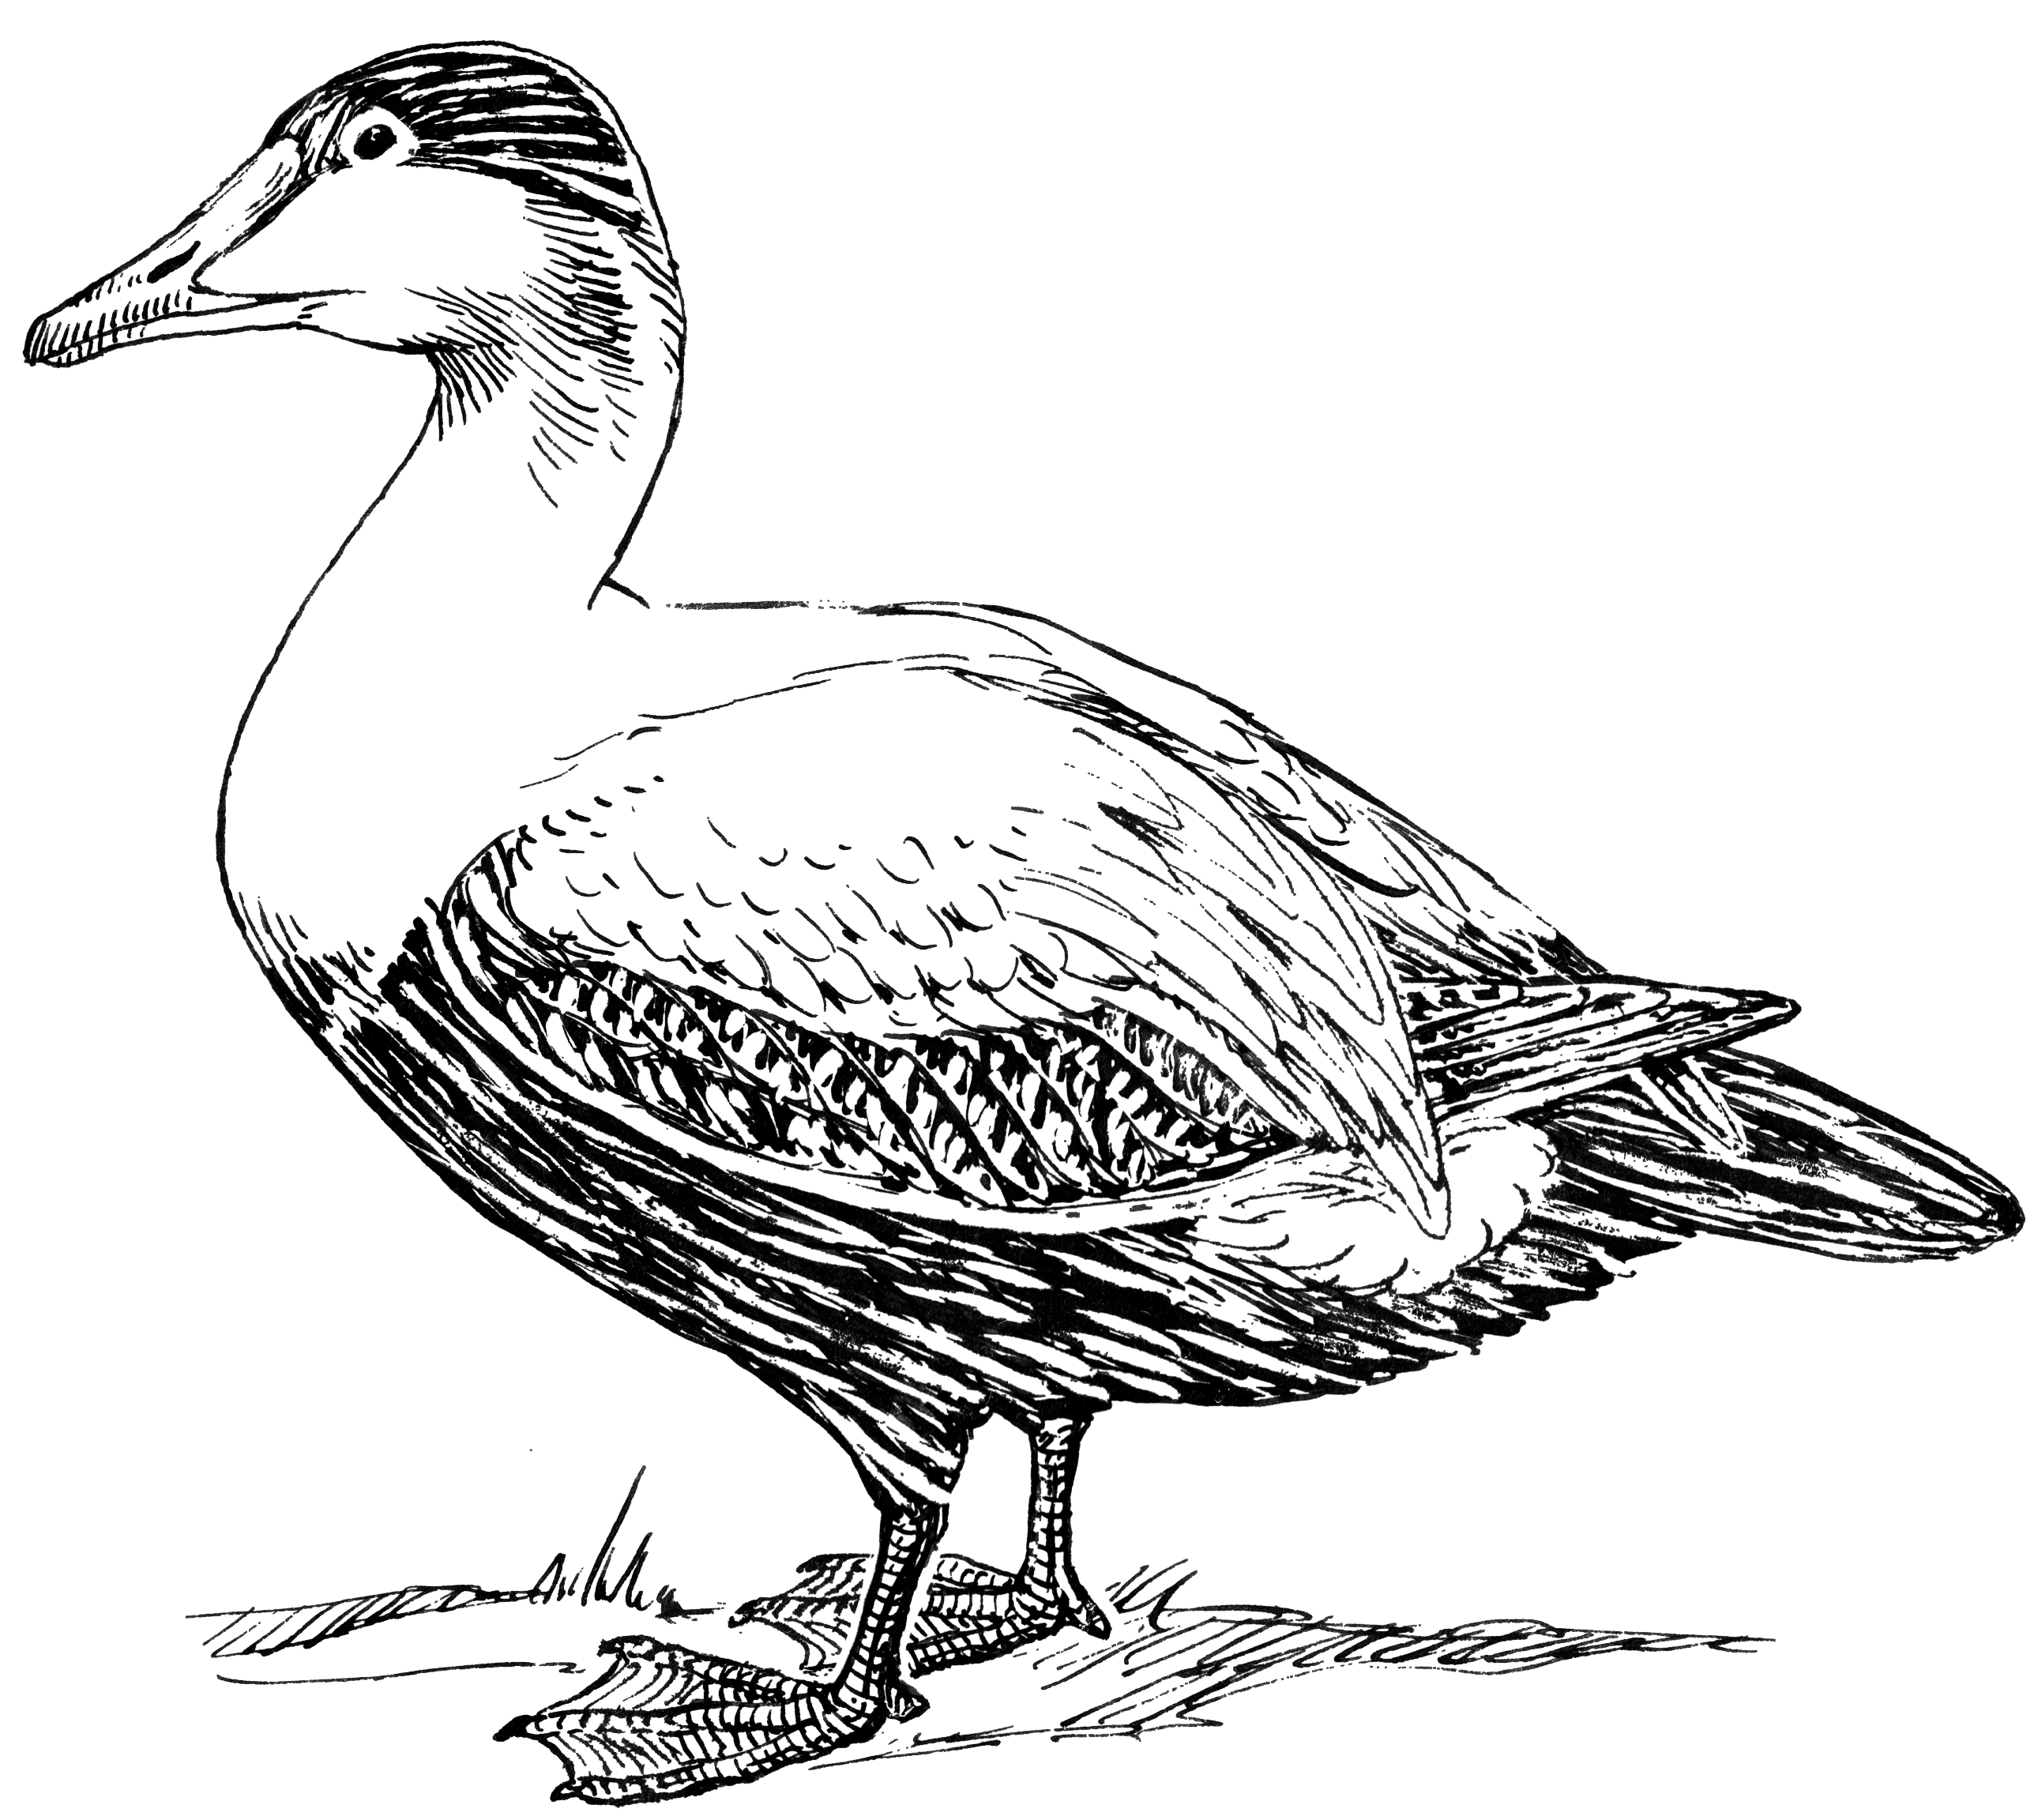
\includegraphics[width=.25\textwidth]{duck}
    
    \textit{If it looks like a duck and quacks like a duck\\ but it needs
    batteries,\\you probably have the wrong abstraction.}
  \end{center}
\end{frame}

\begin{frame}{Things that look like extensionality\dots}
  \begin{block}{Injectivity of constructors}
    \[
    succ(x) \neq succ(y) \lor x = y
    \]
    What happens if we treat this as an extensionality axiom?
  \end{block}
  
  \begin{block}{Solution}
    Exclude clauses with a disequality of the same sort as $x = y$
  \end{block}
\end{frame}

\begin{frame}{Things that look like extensionality\dots}
  \begin{block}{Axiomatization of arrays}
    \[
    i = j \lor select(store(a,i,e), j) = select(a, j)
    \]
  \end{block}

  \begin{block}{Solution}
    Exclude clauses with an equality other than the one among
    variables
  \end{block}
\end{frame}
